% Options for packages loaded elsewhere
\PassOptionsToPackage{unicode}{hyperref}
\PassOptionsToPackage{hyphens}{url}
%
\documentclass[
]{article}
\usepackage{amsmath,amssymb}
\usepackage{iftex}
\ifPDFTeX
  \usepackage[T1]{fontenc}
  \usepackage[utf8]{inputenc}
  \usepackage{textcomp} % provide euro and other symbols
\else % if luatex or xetex
  \usepackage{unicode-math} % this also loads fontspec
  \defaultfontfeatures{Scale=MatchLowercase}
  \defaultfontfeatures[\rmfamily]{Ligatures=TeX,Scale=1}
\fi
\usepackage{lmodern}
\ifPDFTeX\else
  % xetex/luatex font selection
\fi
% Use upquote if available, for straight quotes in verbatim environments
\IfFileExists{upquote.sty}{\usepackage{upquote}}{}
\IfFileExists{microtype.sty}{% use microtype if available
  \usepackage[]{microtype}
  \UseMicrotypeSet[protrusion]{basicmath} % disable protrusion for tt fonts
}{}
\makeatletter
\@ifundefined{KOMAClassName}{% if non-KOMA class
  \IfFileExists{parskip.sty}{%
    \usepackage{parskip}
  }{% else
    \setlength{\parindent}{0pt}
    \setlength{\parskip}{6pt plus 2pt minus 1pt}}
}{% if KOMA class
  \KOMAoptions{parskip=half}}
\makeatother
\usepackage{xcolor}
\usepackage[margin=1in]{geometry}
\usepackage{graphicx}
\makeatletter
\def\maxwidth{\ifdim\Gin@nat@width>\linewidth\linewidth\else\Gin@nat@width\fi}
\def\maxheight{\ifdim\Gin@nat@height>\textheight\textheight\else\Gin@nat@height\fi}
\makeatother
% Scale images if necessary, so that they will not overflow the page
% margins by default, and it is still possible to overwrite the defaults
% using explicit options in \includegraphics[width, height, ...]{}
\setkeys{Gin}{width=\maxwidth,height=\maxheight,keepaspectratio}
% Set default figure placement to htbp
\makeatletter
\def\fps@figure{htbp}
\makeatother
\setlength{\emergencystretch}{3em} % prevent overfull lines
\providecommand{\tightlist}{%
  \setlength{\itemsep}{0pt}\setlength{\parskip}{0pt}}
\setcounter{secnumdepth}{-\maxdimen} % remove section numbering
   \usepackage{setspace}\doublespacing
   \usepackage{booktabs}
   \usepackage{longtable}
   \usepackage{array}
   \usepackage{multirow}
   \usepackage{wrapfig}
   \usepackage{colortbl}
   \usepackage{tabu}
   \usepackage{threeparttable}
   \usepackage{threeparttablex}
   \usepackage[normalem]{ulem}
   \usepackage{makecell}
   \usepackage{xcolor}
   \usepackage{placeins}
   \usepackage{amssymb}
   \renewcommand{\topfraction}{.85}
   \renewcommand{\bottomfraction}{.7}
   \renewcommand{\textfraction}{.15}
   \renewcommand{\floatpagefraction}{.66}
   \setcounter{topnumber}{3}
   \setcounter{bottomnumber}{3}
   \setcounter{totalnumber}{4}
   \usepackage{float}
   \let\origtable\table
   \let\endorigtable\endtable
   \renewenvironment{table}[1][ht]{
      \expandafter\origtable\expandafter[H]
    }{
      \endorigtable
    }
   \usepackage{pdflscape}
   \newcommand{\blandscape}{\begin{landscape}}
    \newcommand{\elandscape}{\end{landscape}}
    \usepackage{adjustbox}
     \setkeys{Gin}{width=\linewidth,height=\textheight,keepaspectratio}

    
\usepackage{booktabs}
\usepackage{longtable}
\usepackage{array}
\usepackage{multirow}
\usepackage{wrapfig}
\usepackage{float}
\usepackage{colortbl}
\usepackage{pdflscape}
\usepackage{tabu}
\usepackage{threeparttable}
\usepackage{threeparttablex}
\usepackage[normalem]{ulem}
\usepackage{makecell}
\usepackage{xcolor}
\ifLuaTeX
  \usepackage{selnolig}  % disable illegal ligatures
\fi
\IfFileExists{bookmark.sty}{\usepackage{bookmark}}{\usepackage{hyperref}}
\IfFileExists{xurl.sty}{\usepackage{xurl}}{} % add URL line breaks if available
\urlstyle{same}
\hypersetup{
  pdftitle={Outline},
  pdfauthor={Shadi},
  hidelinks,
  pdfcreator={LaTeX via pandoc}}

\title{Outline}
\author{Shadi}
\date{2023-08-07}

\begin{document}
\maketitle

\hypertarget{introduction}{%
\subsection{1. Introduction}\label{introduction}}

\hypertarget{background-of-aca}{%
\subsubsection{1.1. Background of ACA}\label{background-of-aca}}

\begin{itemize}
\tightlist
\item
  The Affordable Care Act (ACA) was enacted in 2010 in response to
  failures in the US insurance and healthcare markets, aiming to
  introduce universal health care reform.
\item
  The ACA included various provisions such as insurance reform, health
  insurance exchange establishment, and subsidies to achieve nearly
  universal health insurance
  coverage.{[}@courtemancheEarlyImpactsAffordable2017{]}
\item
  Medicaid Expansion, a crucial ACA provision, was implemented in 2014,
  allowing childless individuals with income below 138\% of the federal
  poverty level (FPL) to apply for Medicaid coverage.Following the
  Supreme Court decision in 2012, states had the option to participate
  in Medicaid Expansion; as of July 2022, 39 states (including DC) have
  implemented it {[}@kaiserfamilyfoundationStatusStateMedicaid2022{]}
\item
  Primary Goals of Medicaid Expansion is goes beyond just enhancing
  access to medical services;and increase in coverage, it also aims to
  address health inequities and reducing the disparities that exist
  among various demographic groups.
\end{itemize}

\hypertarget{problem-statement}{%
\subsubsection{1.2. Problem Statement}\label{problem-statement}}

\begin{itemize}
\tightlist
\item
  Ongoing policy evaluation is necessary even years after implementation
  to ensure that the policy continues to produce the intended outcomes,
  adapt to changing circumstances, and address any unforeseen
  consequences that may have arisen over time.
\item
  Numerous policy analysts and researchers have evaluated the effect of
  Medicaid on variety of desired outcomes, including direct outcome like
  insurance coverage and less direct consequences such as unemployment.
\item
  Many investigated whether the Medicaid expansion's benefits were
  distributed equally across all beneficiary groups.
\item
  One beneficiary groups that hasn't been studied as much as other are
  vulnerable population but is important to include in the literature
  are foreign-borns.

  \begin{itemize}
  \item
    Many of Foreign-born population benefit from Medicaid expansion.
    This include low income, US citizen born abroad , US citizen who
    become citizens through naturalization, and those immigrants that
    are eligible to receive benefits from public program according to
    Personal Responsibility and Work Opportunity Reconciliation
    Act(PRWORA) of 1996..
  \item
    Foreign-born make up a great portion of US population.
  \item
    Foreign-born immigrants are more likely to be low-income.
  \item
    Foreign-born, face additional challenges in access to care
  \end{itemize}
\item
  Understanding how Medicaid expansion impacts these two distinct groups
  is essential for crafting effective policies that address the
  intricate interplay between policy, demographics, and healthcare
  access.
\end{itemize}

\hypertarget{research-gap}{%
\subsubsection{1.3. Research Gap}\label{research-gap}}

While few studies compared the effects of the ACA among foreign-born and
immigrants vs citizen a critical gap persists in the literature.

\begin{enumerate}
\def\labelenumi{\arabic{enumi}.}
\tightlist
\item
  Those that I find are descriptive one can not infer a causal
  relationship
\item
  many are at state level and cannot be generalize to the whole US
  population
\item
  Includes one or at most two years of data after the Medicaid expansion
  went into effect, which is not enough time to see all the outcome of a
  policy change.
\item
  They have not isolate the separate effects of expanding Medicaid
  eligibility versus other changes such as the introduction of market
  plan insurance subsidies
\end{enumerate}

\hypertarget{research-questions-and-hypotheses}{%
\subsubsection{1.4. Research Questions and
Hypotheses}\label{research-questions-and-hypotheses}}

\begin{itemize}
\tightlist
\item
  The central research question guiding this study is: ``How does the
  effect of Medicaid expansion differ between foreign-born and native
  populations in terms of uninsured rates and Medicaid take-up?'' This
  overarching inquiry will be addressed through the following
  interconnected objectives:

  \begin{itemize}
  \tightlist
  \item
    Examine the impact of Medicaid expansion on uninsured rates among
    foreign-born and native populations, identifying potential
    disparities. Assess the disparities in Medicaid enrollment and
    utilization between foreign-born and native individuals following
    Medicaid expansion. Identify and analyze the multifaceted factors
    contributing to variations in healthcare access, Medicaid
    utilization, and barriers to enrollment within these demographic
    segments.
  \end{itemize}
\item
  Hypothesis 1: The effect of Medicaid expansion on reducing uninsured
  rates will differ significantly between foreign-born and native
  populations due to an intricate interplay of demographic,
  socio-economic, and cultural factors.
\item
  Hypothesis 2: Foreign-born individuals will exhibit a lower propensity
  for Medicaid take-up post-expansion compared to native individuals,
  attributed to an amalgamation of linguistic, cultural, and
  immigration-related complexities.
\end{itemize}

\hypertarget{theoretical-model}{%
\subsection{2. Theoretical Model}\label{theoretical-model}}

\hypertarget{understanding-rational-for-enrolling-in-medicaid}{%
\subsubsection{2.1. Understanding Rational for Enrolling in
Medicaid}\label{understanding-rational-for-enrolling-in-medicaid}}

\begin{itemize}
\item
  \textbf{Conventional health insurance theory}: Individual are risk
  averse, thus purchase insurance to reduce risk of large loss. Free or
  subsidized insurance like medicaid increase the insurance demand,
  increase the risky behavior, increase health care use and reduces
  welfare.
\item
  \textbf{Nyman Theory of Insurance Demand}: Not all individual are risk
  averse, individual purchase insurance to gain additional income for
  their time of illness. Offer of free insurance, increase demand for
  insurance, increase the use of healthcare, increase the social
  welfare.
\item
  Both Nyman Theory and Conventional health insurance theory are based
  on rational choice theory.They predict that free or subsidized
  insurance will increase the demand for the insurance and health care.
  From Nyman's theory we infer that expanding Medicaid, can improve
  healthcare utilization and outcomes, but practical challenges
  complicate this theoretical alignment.
\item
  Empirical evidence shows imperfect uptake of social benefits,
  diverging from expected theoretical outcomes. Some Medicaid-eligible
  individuals do not claim entitled benefits (Wehby \& Lyu, 2018).
  Non-utilization of benefits extends globally beyond Medicaid and the
  US population. Some effectively use social assistance while others do
  not.
\item
  Non-utilization's significance reaches beyond healthcare access,
  promoting equitable outcomes.
\end{itemize}

\hypertarget{exploring-models-that-explains-take-up-pattern-of-social-welfare}{%
\subsubsection{2.2. Exploring Models That Explains Take-Up Pattern of
Social
Welfare}\label{exploring-models-that-explains-take-up-pattern-of-social-welfare}}

\begin{itemize}
\tightlist
\item
  Additional theories and perspectives are crucial to understanding
  non-utilization complexities.
\item
  The literature on social welfare program participation, like Medicaid,
  encompasses two key perspectives: traditional economics, which relies
  on rational choice theory, and behavioral economics, which emphasizes
  cognitive barriers to decision-making.
\item
  Van Oorschot's Multilevel System Model: provides a valuable
  overarching framework that ties together various models and factors
  that offers a comprehensive lens by examining factors across multiple
  levels.

  \begin{itemize}
  \tightlist
  \item
    Considers personal motivations, administrative procedures, and
    policy contexts as intertwined influences on benefit uptake.
  \item
    Allows for analyzing the interplay between individual,
    administrative, and policy-level factors in Medicaid insurance
    utilization.
  \end{itemize}
\end{itemize}

\hypertarget{foreign-born-vs.-native-populations-a-comparative-approach}{%
\subsubsection{2.3. Foreign-Born vs.~Native Populations: A Comparative
Approach:}\label{foreign-born-vs.-native-populations-a-comparative-approach}}

\begin{itemize}
\tightlist
\item
  Contradictory empirical evidence exists on social benefit uptake rates
  among immigrants and native-born individuals.
\item
  There is uncertainty about whether foreign-born uptake rates are
  higher, lower, or equivalent.
\item
  Leveraging Van Oorschot's model, I comprehensively examine factors
  influencing benefit uptake.
\end{itemize}

\hypertarget{analyzing-factors-affecting-uptake-among-foreign-born-individuals-using-van-oorschots-model.}{%
\subsubsection{2.4. Analyzing Factors Affecting Uptake Among
Foreign-born Individuals Using Van Oorschot's
Model.}\label{analyzing-factors-affecting-uptake-among-foreign-born-individuals-using-van-oorschots-model.}}

\hypertarget{individual-level-factors}{%
\paragraph{2.4.1. Individual Level
Factors:}\label{individual-level-factors}}

\begin{itemize}
\tightlist
\item
  \emph{Perceived Deservingness}, foreign-born individuals' perception
  of entitlement to social benefits based on contributions and
  circumstances.
\item
  \emph{Institutional Trust}, Trust in host country institutions'
  fairness and reliability regarding benefit provision.
\item
  \emph{Language Proficiency}, Influence of language skills on benefit
  comprehension and access.
\item
  \emph{Social Networks}, Impact of personal networks on benefit
  enrollment decisions.
\item
  \emph{Cultural Perceptions and Stigma}, Role of cultural beliefs and
  stigma in public assistance choices.
\item
  \emph{Integration Level}, how integration into the host society
  affects benefit knowledge and utilization.
\item
  \emph{Unfamiliarity with Local Resources} Challenges due to
  unfamiliarity with local services for accessing benefits.
\end{itemize}

\hypertarget{administrative-level}{%
\paragraph{2.4.2. Administrative Level:}\label{administrative-level}}

\begin{itemize}
\tightlist
\item
  \emph{Complexities of Procedures and Requirements}: Administrative
  hurdles faced by foreign-born individuals due to procedural
  complexities and additional documentation.
\item
  \emph{Administrator Prejudice}: Bias from administrators based on
  classicism towards immigrants affecting benefit access.
\end{itemize}

\pagebreak

\hypertarget{policy-level}{%
\paragraph{2.4.3. Policy Level:}\label{policy-level}}

\begin{itemize}
\tightlist
\item
  \emph{Chilling Effect of Policies}: The discouraging impact of
  policies like immigration enforcement and public charge rule on
  seeking benefits.
\item
  \emph{Outreach Programs}: Effectiveness of outreach initiatives
  targeting foreign-born individuals for benefit awareness.
\item
  \emph{Political Climate and Discourse}: Influence of political context
  and public discourse on policies related to foreign-born populations.
\end{itemize}

Drawing from our theoretical insights, we detail data sources, analysis
methods, and controls, bridging theoretical concepts with rigorous
empirical investigation.

\hypertarget{emprical-strategy}{%
\subsection{3. Emprical Strategy}\label{emprical-strategy}}

\hypertarget{data}{%
\subsubsection{3.1. Data}\label{data}}

\hypertarget{sources}{%
\paragraph{3.1.1. Sources}\label{sources}}

\begin{itemize}
\tightlist
\item
  American Community Survey (ACS) which is accessible via the Public Use
  Microdata Sample(PUMS)
\item
  Kaiser Family Foundation(KFF) State's Health Facts for the dynamic
  status of medicaid expansion.
\end{itemize}

\hypertarget{sample-restrictions}{%
\paragraph{3.1.2. Sample Restrictions}\label{sample-restrictions}}

\begin{itemize}
\item
  To ensure the internal validity of our study and focus on individuals
  more likely to be eligible for Medicaid, I have carefully established
  the following sample restrictions:
\item
  Age Inclusion (26-65):Include individuals aged 26 to 65 to exclude
  ACA's young adult provision and Medicare-eligible individuals.
\item
  Income Threshold (less than138\% FPL):Select individuals with incomes
  at below 138\% FPL, aligning with Medicaid eligibility criteria.
\item
  Exclude non-citizens less than 5 years adhering to Lawfully Present
  Immigrants' waiting period. Recognize data limitations regarding
  immigration status/visa types.
\item
  Excluded non-citizens who have been residing in U.S. for less than
  five years. since Lawfully Present Immigrants should wait five year to
  qualify for Medicaid. Some limitation Immigration status/ visa type is
  not declreaed in dataset. Refugees and Asylees are not subject to the
  5 year bar. Undocumented are on eligible for Medicaid. Some states
  waived the requirments.
\item
  Time Frame (2011-2019): To avoid ACA's minor provisions in 2010 and
  COVID-19 complexities in 2020
\item
  Remove states with similar policies for a focused analysis of Medicaid
  expansion effects.
\item
  Exclude individuals in prisons, nursing homes, mental hospitals, etc.
  since ACS lacks information on poverty Measures:
\end{itemize}

\hypertarget{measures}{%
\subsubsection{3.2. Measures}\label{measures}}

\begin{itemize}
\item
  \textbf{Treatment}: \emph{Medicaid Expansion Status}, binary variable
  indicating states' decision to expand Medicaid (0 for non-expansion, 1
  for expansion during 2014-2020).
\item
  \textbf{Outcome}: \emph{Uninsured Rates}, binary variables derived
  from ACS responses on being insurancd during previous year.
  \emph{Medicaid Coverage} another binary variables derived from ACS
  responses on having Medicaid coverage during the previous year.
\item
  \textbf{Nativity Status}: binary variable distinguishing individuals
  as ``Native'' (1) if born in the U.S. or its territories, and
  ``Foreign-Born'' (0) if born outside the U.S.
\item
  \textbf{Demographic Characteristics}: \emph{Age}, \emph{gender},
  \emph{marital status}, \emph{race}, and \emph{ethnicity}.
\item
  \textbf{Socioeconomic Factors}: \emph{Income}, \emph{education},
  \emph{employment status}.
\item
  \textbf{Disability Status}:Binary variable indicating disability
  status.
\item
  \textbf{Foreign-Born Specific Variables}: \emph{Language Proficiency},
  \emph{Length of Residency}, \emph{Region of Origin}. \emph{Citizenship
  Status}, a binary variable showing if a person is citizen or
  non-Citizen.
\item
  \textbf{State-Level Measures:} \emph{Immigration Policy Climate (IPC)
  Index}, reflecting immigration policy friendliness or restrictiveness.
  \emph{Unemployment Rate}, indicating economic conditions.
  \emph{Americans for Democratic Action (ADA) Scores}, measuring state
  legislators' perceived liberalism.
\end{itemize}

\hypertarget{methodology}{%
\subsubsection{3.3. Methodology}\label{methodology}}

\hypertarget{difference-in-differences-did-estimation}{%
\paragraph{3.3.1. Difference-in-Differences (DID)
Estimation:}\label{difference-in-differences-did-estimation}}

\begin{itemize}
\tightlist
\item
  DID is used to estimate the impact of Medicaid expansion on Uninsured
  and Medicaid Coverage.
\item
  Utilizing a two-way fixed effects model with differential timing,
  which enables the incorporation of the Medicaid expansion timeline
  into the DID analysis.
\end{itemize}

\textbf{Model Specification:}

\begin{equation}
Y_{ist} = \alpha + \delta_s + \lambda_t + \gamma_s \cdot Treat_{st} + \beta_1 (FB_{ist} \times Treat_{st}) + FB_{ist} + \beta  X_{ist} + \theta(FB_{ist} \times C_{ist}) + \epsilon_{ist}
\end{equation}

\textbf{Equation Components:}

\begin{itemize}
\tightlist
\item
  \(Y_{ist}\) represents the outcome of individual \(i\) in year \(t\)
  in state \(s\).
\item
  \(\delta_s\) represents state fixed effects.
\item
  \(\lambda_t\) represents year fixed effects.
\item
  \(\gamma\) represents the average treatment effect of Medicaid
  expansion for state \(s\).
\item
  \(Treat_{st}\) is a dummy variable that equals 1 if individual \(i\)
  in state \(s\) is exposed to the treatment in year \(t\), and 0
  otherwise. For states that expanded Medicaid in 2014, \(Treat_{st}\)
  is equal to 1 for all years after 2014. For states that expanded
  Medicaid later, \(T_{ist}\) is equal to 1 for all years after the year
  of expansion.
\item
  \(\beta_1\) represents the coefficient for the interaction term
  between \(FB_{ist}\) and \(T_{st}\), capturing the differential
  treatment effect for foreign-born individuals. X represents vector of
  control variables, including racial composition, age distribution,
  gender distribution, employment, and personal income
\item
  \(\theta_k \cdot (FB_{ist} \times C_{ist,k})\) represents the
  interaction terms between the binary variable \(FB_{ist}\) and the
  control variables specifice to foreign-born individuals
  (\(C_{ist,k}\)). These interaction terms capture the differential
  effects of the control variables for foreign-born individuals compared
  to native-born individuals.
\end{itemize}

The standard errors are adjusted to accommodate for serial correlation
at the state level and heteroskedastic errors.

\hypertarget{event-study-estimation}{%
\paragraph{3.3.2. Event Study
Estimation:}\label{event-study-estimation}}

\begin{itemize}
\item
  Additionally, I estimate this effect using an event study model that
  allows us to assess the evolution of relative outcomes while
  controlling for fixed differences across states and national trends
  over time.
\item
  Event study model allows us to test the parallel trends assumption and
  it provides valuable insights into the temporal dynamics of the
  treatment effect, enhancing our understanding of the causal
  relationship between the treatment and the outcome variable.
\end{itemize}

\textbf{Model Specification:}

\begin{equation}
{Y}_{its}=  {\alpha} + {\delta}_s + {\lambda}_t+{\psi}{X}_{ist} + \sum_{k=-4,k\neq -1}^{6} {\beta}_k{D}_{k,its} 
 +{\epsilon}_{its}.
\end{equation}

\textbf{Equation Components:}

\begin{itemize}
\tightlist
\item
  \(Y_{ist}\): Outcome for individual \(i\) each year and state.
\item
  \(\delta_s\): State fixed effect.
\item
  \(\lambda_t\): Year fixed effects.
\item
  \(X_{idt}\): Vector of control variables.
\end{itemize}

\textbf{Dynamic Policy Effects:}

\begin{itemize}
\tightlist
\item
  \(\sum_{n=-3}^{5} \beta_y D_s D_{it}^n\): Captures dynamic effects of
  policy.
\item
  \(D_{k,its}\): Lead and lag dummy variables when state adopts
  expansion.
\item
  \({\beta}_y\): Estimates change in outcomes in expansion
  vs.~non-expansion states during year \(y\).
\end{itemize}

\textbf{Omitted Category:}

\begin{itemize}
\tightlist
\item
  \(k=-1\): Year prior to expansion, excluded as omitted category.
\end{itemize}

\hypertarget{addressing-challenges-of-varying-treatment-effects-over-time-in-the-literature}{%
\paragraph{3.3.3 Addressing challenges of varying treatment effects over
time in the
literature:}\label{addressing-challenges-of-varying-treatment-effects-over-time-in-the-literature}}

\begin{itemize}
\tightlist
\item
  Recent research in econometrics has raised concerns about the
  potential bias in staggered difference-in-differences and event
  studies estimates when treatment effects are heterogeneous and
  treatment timing varies across units.
\item
  This research is susceptible to these concerns since some states
  implemented Medicaid expansions after 2014, making the timing of
  treatment heterogeneous across units.
\item
  To address these challenge I used :

  \begin{itemize}
  \tightlist
  \item
    Interaction-weighted (IW) event study estimator proposed by Sun \&
    Abraham (2021)
  \item
    Bacon decomposition and examine the consistency of the results.
  \end{itemize}
\end{itemize}

\hypertarget{result}{%
\subsection{4. Result}\label{result}}

\hypertarget{causal-structure-discovery}{%
\subsubsection{4.1. Causal Structure
Discovery}\label{causal-structure-discovery}}

\begin{itemize}
\item
  Employed causal structure discovery techniques to construct a complex
  DAG from the data itself. to capture variable interactions, account
  for confounding factors and biases, provide credible evidence for
  Medicaid expansion effects.
\item
  The DAG generated using multiple constraint-based and score-based
  algorithms including GDS algorithms, Greedy Equivalence Search (GES),
  Peter-Clark (PC) algorithm, and Fast Causal Inferences (FCI).
\item
  Obtained a final graph using the majority voting approach following
  Joe et al.(2023)
\item
  Carefully reviewed and adjusted the graph to align better with
  real-world expertise, simplifying complex relationships.
\item
  The derived DAG served as a valuable tool for generating hypotheses
  and guiding the analysis process.AND helped in selecting relevant
  control variables for the analysis based on the identified
  relationships.
\end{itemize}

\begin{center}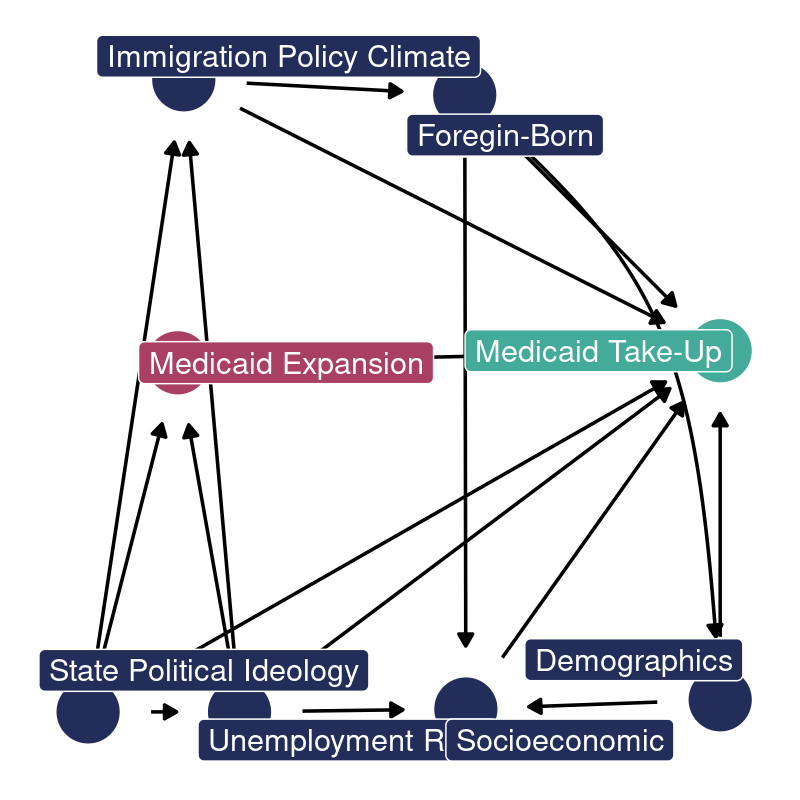
\includegraphics{/home/shadi/Projects/GitHub/medicaid-foreign-born/output/DAG3-1} \end{center}

\hypertarget{descriptive-results}{%
\subsubsection{4.2. Descriptive Results}\label{descriptive-results}}

Table 1 provides a baseline comparison of Non-Expansion and Expansion
states before and after the implementation of the Affordable Care Act
(ACA). The table displays mean values for three variables: State's
Political Liberalism, Immigration Policy Climate, and State's
Unemployment Rate.

\begin{table}[H]

\caption{\label{tab:tab1}Baseline Comparison of States}
\centering
\begin{tabular}[t]{>{}llccc}
\toprule
\textbf{Group} & \textbf{Variable} & \textbf{Expansion} & \textbf{Non Expansion} & \textbf{Difference}\\
\midrule
\textbf{Pre-ACA} & State's Political Liberalism & 0.45 (0.17) & 0.24 (0.09) & \textbf{0.22***}\\
\textbf{} & Immigration Policy Climate & -1 (2) & -3 (1) & \textbf{2.1***}\\
\textbf{} & State's Unemployment Rate & 8.60 (1.64) & 7.16 (2.02) & \textbf{1.4***}\\
\midrule
\textbf{Post-ACA} & State's Political Liberalism & 0.47 (0.22) & 0.23 (0.10) & \textbf{0.24***}\\
\textbf{} & Immigration Policy Climate & 0 (3) & -3 (1) & \textbf{2.8***}\\
\textbf{} & State's Unemployment Rate & 5.00 (1.14) & 4.50 (1.15) & \textbf{0.50***}\\
\bottomrule
\multicolumn{5}{l}{\rule{0pt}{1em}\textsuperscript{1} Mean (SD)}\\
\multicolumn{5}{l}{\rule{0pt}{1em}\textsuperscript{2} \textit{p<0.05; \textbf{p<0.01; }}p<0.001}\\
\end{tabular}
\end{table}

\textbf{Key Observations:}

\begin{itemize}
\tightlist
\item
  Before the ACA went into effect, there were notable differences
  between Expansion and Non-Expansion states.
\item
  Expansion states tended to be more politically liberal.
\item
  Expansion states had less exclusionary immigration policies.
\item
  Expansion states had higher levels of unemployment.
\item
  Implementation of the ACA did not significantly impact the differences
  in State's Political Liberalism, Immigration Policy Climate, and
  State's Unemployment Rate between Expansion and Non-Expansion states.
\end{itemize}

Table 2 gives a detailed look at demographics, insurance rates, and
Medicaid coverage before the Affordable Care Act. It compares
foreign-born and US-born individuals in states with and without Medicaid
expansion.

\begin{table}[H]

\caption{\label{tab:tab2}Baseline Characteristics by Nativity}
\centering
\resizebox{\linewidth}{!}{
\begin{tabular}[t]{lcccccc}
\toprule
\multicolumn{1}{c}{ } & \multicolumn{3}{c}{\textbf{Expansion}} & \multicolumn{3}{c}{\textbf{Non-expansion}} \\
\cmidrule(l{3pt}r{3pt}){2-4} \cmidrule(l{3pt}r{3pt}){5-7}
\textbf{Characteristic} & \makecell[c]{\textbf{Foregin-born}, \\N = 11592215} & \makecell[c]{\textbf{US-born}, \\N = 34946509} & \textbf{p-value} & \makecell[c]{\textbf{Foregin-born}, \\N = 7113051} & \makecell[c]{\textbf{US-born}, \\N = 26041282} & \textbf{p-value}\\
\midrule
\textbf{Uninsured, \%} & 56 & 34 & <0.001 & 70 & 42 & <0.001\\
\textbf{Medicaid coverage, \%} & 25 & 38 & <0.001 & 12 & 30 & <0.001\\
\textbf{Age, Mean (SD)} & 42 (10) & 44 (11) & <0.001 & 41 (10) & 44 (11) & <0.001\\
\textbf{Race/ethnicity, \%} &  &  & <0.001 &  &  & <0.001\\
\hspace{1em}Asian & 15 & 0.8 &  & 7.3 & 0.2 & \\
\hspace{1em}Black & 4.3 & 20 &  & 7.9 & 28 & \\
\hspace{1em}Hispanic & 68 & 11 &  & 76 & 10 & \\
\hspace{1em}Other & 1.8 & 4.3 &  & 1.5 & 3.2 & \\
\hspace{1em}White & 11 & 64 &  & 7.6 & 58 & \\
\textbf{Sex, \%} &  &  & <0.001 &  &  & <0.001\\
\hspace{1em}Female & 55 & 57 &  & 54 & 58 & \\
\hspace{1em}Male & 45 & 43 &  & 46 & 42 & \\
\textbf{Married, \%} & 56 & 28 & <0.001 & 58 & 31 & <0.001\\
\textbf{Employment status, \%} &  &  & <0.001 &  &  & <0.001\\
\hspace{1em}Employed & 53 & 38 &  & 57 & 40 & \\
\hspace{1em}Not in labor force & 35 & 47 &  & 33 & 46 & \\
\hspace{1em}Unemployed & 11 & 15 &  & 9.8 & 14 & \\
\textbf{Education, \%} &  &  & <0.001 &  &  & <0.001\\
\hspace{1em}College degree & 6.9 & 8.2 &  & 6.6 & 7.2 & \\
\hspace{1em}Graduate and beyond & 2.8 & 2.8 &  & 2.4 & 2.2 & \\
\hspace{1em}High school & 24 & 36 &  & 26 & 36 & \\
\hspace{1em}Less than high school & 51 & 20 &  & 50 & 22 & \\
\hspace{1em}Some college or Associate degree & 15 & 33 &  & 15 & 32 & \\
\textbf{Federal poverty, \%} &  &  & <0.001 &  &  & <0.001\\
\hspace{1em}Income\ \ 100 to 138\% poverty & 37 & 31 &  & 36 & 32 & \\
\hspace{1em}Income below 100\% poverty & 63 & 69 &  & 64 & 68 & \\
\textbf{Disability, \%} & 9.8 & 27 & <0.001 & 9.3 & 27 & <0.001\\
\bottomrule
\multicolumn{7}{l}{\rule{0pt}{1em}\textsuperscript{1} chi-squared test with Rao \& Scott's second-order correction; Wilcoxon rank-sum test for complex survey samples}\\
\end{tabular}}
\end{table}

\textbf{Key Observations:}

\begin{itemize}
\tightlist
\item
  Notable demographic variations exist when comparing foreign-born and
  US-born adults, regardless of Medicaid expansion status.
\item
  Baseline data shows minimal or negligible differences in
  characteristics of foreign-born individuals between expansion and
  non-expansion states.
\item
  At the baseline, characteristics of native-born individuals exhibit
  either no differences or slight variations between expansion and
  non-expansion states.
\end{itemize}

Table 3, provides a comprehensive view of uninsured individuals'
characteristics, along with those covered by Medicaid, before and after
the implementation of the Affordable Care Act (ACA) in both Medicaid
expansion and non-expansion states.

It shows changes in uninsured and Medicaid-covered groups post-ACA. and
provides context on the ACA's impact across different state contexts.

\begin{table}

\caption{\label{tab:tab3}Charachterstics of Uninsured and Medicaid Covered Low Income Indiduals, expansion vs non-expansion}
\centering
\fontsize{8}{10}\selectfont
\begin{tabular}[t]{lcccccccc}
\toprule
\multicolumn{1}{c}{ } & \multicolumn{4}{c}{Uninsured Rate} & \multicolumn{4}{c}{Medicaid Coverage} \\
\cmidrule(l{3pt}r{3pt}){2-5} \cmidrule(l{3pt}r{3pt}){6-9}
\multicolumn{1}{c}{ } & \multicolumn{2}{c}{Expansion} & \multicolumn{2}{c}{Non-expansion} & \multicolumn{2}{c}{Expansion} & \multicolumn{2}{c}{Non-expansion} \\
\cmidrule(l{3pt}r{3pt}){2-3} \cmidrule(l{3pt}r{3pt}){4-5} \cmidrule(l{3pt}r{3pt}){6-7} \cmidrule(l{3pt}r{3pt}){8-9}
Characteristic & Pre & Post & Pre & Post & Pre & Post & Pre & Post\\
\midrule
\textbf{Nativity, \%} &  &  &  &  &  &  &  & \\
\hspace{1em}Foregin-born & 36 & 32 & 28 & 27 & 17 & 17 & 9.1 & 8.8\\
\hspace{1em}US-born & 64 & 68 & 72 & 73 & 83 & 83 & 91 & 91\\
\textbf{Race/ethnicity, \%} &  &  &  &  &  &  &  & \\
\hspace{1em}Asian & 3.8 & 4.2 & 1.7 & 1.9 & 4.2 & 3.7 & 1.1 & 0.9\\
\hspace{1em}Black & 10 & 11 & 17 & 19 & 14 & 17 & 28 & 31\\
\hspace{1em}Hispanic & 35 & 31 & 32 & 29 & 19 & 19 & 14 & 13\\
\hspace{1em}Other & 6.1 & 4.9 & 3.8 & 3.4 & 5.8 & 6.1 & 4.0 & 3.9\\
\hspace{1em}White & 45 & 49 & 46 & 46 & 56 & 54 & 54 & 51\\
\textbf{Sex, \%} &  &  &  &  &  &  &  & \\
\hspace{1em}Female & 50 & 52 & 55 & 55 & 61 & 63 & 63 & 64\\
\hspace{1em}Male & 50 & 48 & 45 & 45 & 39 & 37 & 37 & 36\\
\textbf{Employment status, \%} &  &  &  &  &  &  &  & \\
\hspace{1em}Employed & 49 & 46 & 48 & 47 & 34 & 27 & 25 & 22\\
\hspace{1em}Not in labor force & 39 & 34 & 40 & 35 & 56 & 60 & 67 & 67\\
\hspace{1em}Unemployed & 12 & 19 & 12 & 18 & 9.9 & 13 & 7.6 & 11\\
\textbf{Marital status, \%} & 35 & 37 & 37 & 39 & 32 & 33 & 29 & 30\\
\textbf{Education, \%} &  &  &  &  &  &  &  & \\
\hspace{1em}College degree & 6.9 & 6.8 & 5.9 & 6.1 & 6.7 & 4.6 & 5.1 & 4.0\\
\hspace{1em}Graduate and beyond & 2.4 & 2.1 & 1.8 & 1.7 & 2.2 & 1.3 & 1.5 & 1.1\\
\hspace{1em}High school & 34 & 34 & 36 & 35 & 35 & 35 & 37 & 35\\
\hspace{1em}Less than high school & 33 & 31 & 32 & 32 & 25 & 30 & 28 & 32\\
\hspace{1em}Some college or Associate degree & 23 & 26 & 25 & 26 & 30 & 29 & 29 & 27\\
\textbf{Federal poverty, \%} &  &  &  &  &  &  &  & \\
\hspace{1em}Income\ \ 100 to 138\% poverty & 32 & 32 & 30 & 31 & 28 & 25 & 26 & 25\\
\hspace{1em}Income below 100\% poverty & 68 & 68 & 70 & 69 & 72 & 75 & 74 & 75\\
\textbf{Disability, \%} & 12 & 13 & 16 & 15 & 34 & 40 & 45 & 48\\
\bottomrule
\end{tabular}
\end{table}

Table 4 presents the shifts in characteristics unique to foreign-born
individuals before and after the enactment of the Affordable Care Act
(ACA) in both Medicaid expansion and non-expansion states.

\begin{table}[H]

\caption{\label{tab:tab4}Changes in Foreign-Born-Specific Characteristics Before and After the Affordable Care Act (ACA) in Expansion and Non-Expansion States}
\centering
\resizebox{\linewidth}{!}{
\fontsize{6.5}{8.5}\selectfont
\begin{tabular}[t]{lcccccc}
\toprule
\multicolumn{1}{c}{ } & \multicolumn{3}{c}{\textbf{Expansion}} & \multicolumn{3}{c}{\textbf{Non-expansion}} \\
\cmidrule(l{3pt}r{3pt}){2-4} \cmidrule(l{3pt}r{3pt}){5-7}
\textbf{Characteristic} & \textbf{Pre-ACA} & \textbf{Post-ACA} & \textbf{Difference} & \textbf{Pre-ACA} & \textbf{Post-ACA} & \textbf{Difference}\\
\midrule
\addlinespace[0.3em]
\multicolumn{7}{l}{\textbf{Insurance coverage, \%}}\\
\hspace{1em}Uninsured & 53 & 33 & 20\%*** & 67 & 54 & 13\%***\\
\hspace{1em}Medicaid coverage & 27 & 43 & -17\%*** & 14 & 16 & -2.7\%***\\
\hspace{1em}Individualy Purchased & 5.4 & 8.3 & -2.9\%*** & 5.0 & 13 & -8.0\%***\\
\hspace{1em}Employer Sponsered & 15 & 16 & -0.90\%*** & 14 & 17 & -3.0\%***\\
\addlinespace[0.3em]
\multicolumn{7}{l}{\textbf{Citizenship status, \%}}\\
\hspace{1em}Naturalized citizen & 33 & 38 & -5.0\%*** & 29 & 34 & -4.5\%***\\
\hspace{1em}Non citizen & 63 & 58 & 5.7\%*** & 66 & 61 & 5.3\%***\\
\hspace{1em}US citizen Born abroad & 3.3 & 4.0 & -0.68\%*** & 4.3 & 5.1 & -0.85\%***\\
\addlinespace[0.3em]
\multicolumn{7}{l}{\textbf{Lifetime in US, \%}}\\
\hspace{1em}Less than 25\% & 17 & 14 & 3.2\%*** & 20 & 16 & 3.7\%***\\
\hspace{1em}More than 25\% & 83 & 86 & -3.2\%*** & 80 & 84 & -3.7\%***\\
\addlinespace[0.3em]
\multicolumn{7}{l}{\textbf{Self-rated English proficiency, \%}}\\
\hspace{1em}Not at all & 16 & 13 & 2.6\%*** & 16 & 14 & 1.7\%***\\
\hspace{1em}Not well & 32 & 29 & 3.4\%*** & 30 & 27 & 2.8\%***\\
\hspace{1em}Only english & 9.6 & 11 & -1.8\%*** & 12 & 13 & -1.2\%***\\
\hspace{1em}Very well & 19 & 23 & -3.7\%*** & 20 & 22 & -2.6\%***\\
\hspace{1em}Well & 23 & 24 & -0.56\%** & 22 & 23 & -0.66\%**\\
\addlinespace[0.3em]
\multicolumn{7}{l}{\textbf{Country/Region of birth, \%}}\\
\hspace{1em}Canada & 1.0 & 1.0 & -0.07\% & 1.1 & 1.0 & 0.07\%\\
\hspace{1em}Eastern Asia & 5.8 & 6.5 & -0.72\%*** & 2.3 & 2.9 & -0.53\%***\\
\hspace{1em}Eastern Europe & 2.3 & 2.4 & -0.12\% & 1.2 & 1.2 & -0.05\%\\
\hspace{1em}Latin America & 68 & 64 & 4.1\%*** & 80 & 77 & 2.7\%***\\
\hspace{1em}Middle East & 3.8 & 4.8 & -1.0\%*** & 1.9 & 2.4 & -0.47\%***\\
\hspace{1em}Oceania and at Sea & 0.6 & 0.7 & -0.04\% & 0.3 & 0.3 & -0.01\%\\
\hspace{1em}South Centeral Asia & 2.6 & 3.5 & -0.87\%*** & 2.1 & 2.5 & -0.38\%***\\
\hspace{1em}South East Asia & 9.5 & 9.9 & -0.33\%** & 4.5 & 5.0 & -0.54\%***\\
\hspace{1em}Sub Saharan Africa & 2.4 & 3.0 & -0.65\%*** & 2.1 & 2.7 & -0.51\%***\\
\hspace{1em}Western Europe & 3.7 & 4.1 & -0.33\%*** & 4.3 & 4.6 & -0.28\%*\\
\bottomrule
\multicolumn{7}{l}{\rule{0pt}{1em}\textsuperscript{1} \%}\\
\multicolumn{7}{l}{\rule{0pt}{1em}\textsuperscript{2} \textit{p<0.05; \textbf{p<0.01; }}p<0.001}\\
\end{tabular}}
\end{table}

\textbf{Key Observations:}

\begin{itemize}
\tightlist
\item
  With the exception of insurance coverage, the foreign-born-specific
  characteristics remain consistent over time and exhibit minimal
  differences between expansion and non-expansion states.
\end{itemize}

\hypertarget{event-study}{%
\subsubsection{4.3. Event Study}\label{event-study}}

\hypertarget{uninsured-rate}{%
\paragraph{4.3.1. Uninsured Rate:}\label{uninsured-rate}}

In Figure 1, Event-study estimates for uninsured rates are displayed.

Panel (a): Focuses on expansion effects on uninsured for both US-born
and foreign-born individuals without control variables. Panel (b):
Examines expansion effects while controlling for covariates. Black line
with circles: Represents foreign-borns. Purple line with triangles:
Represents US-born.

\begin{center}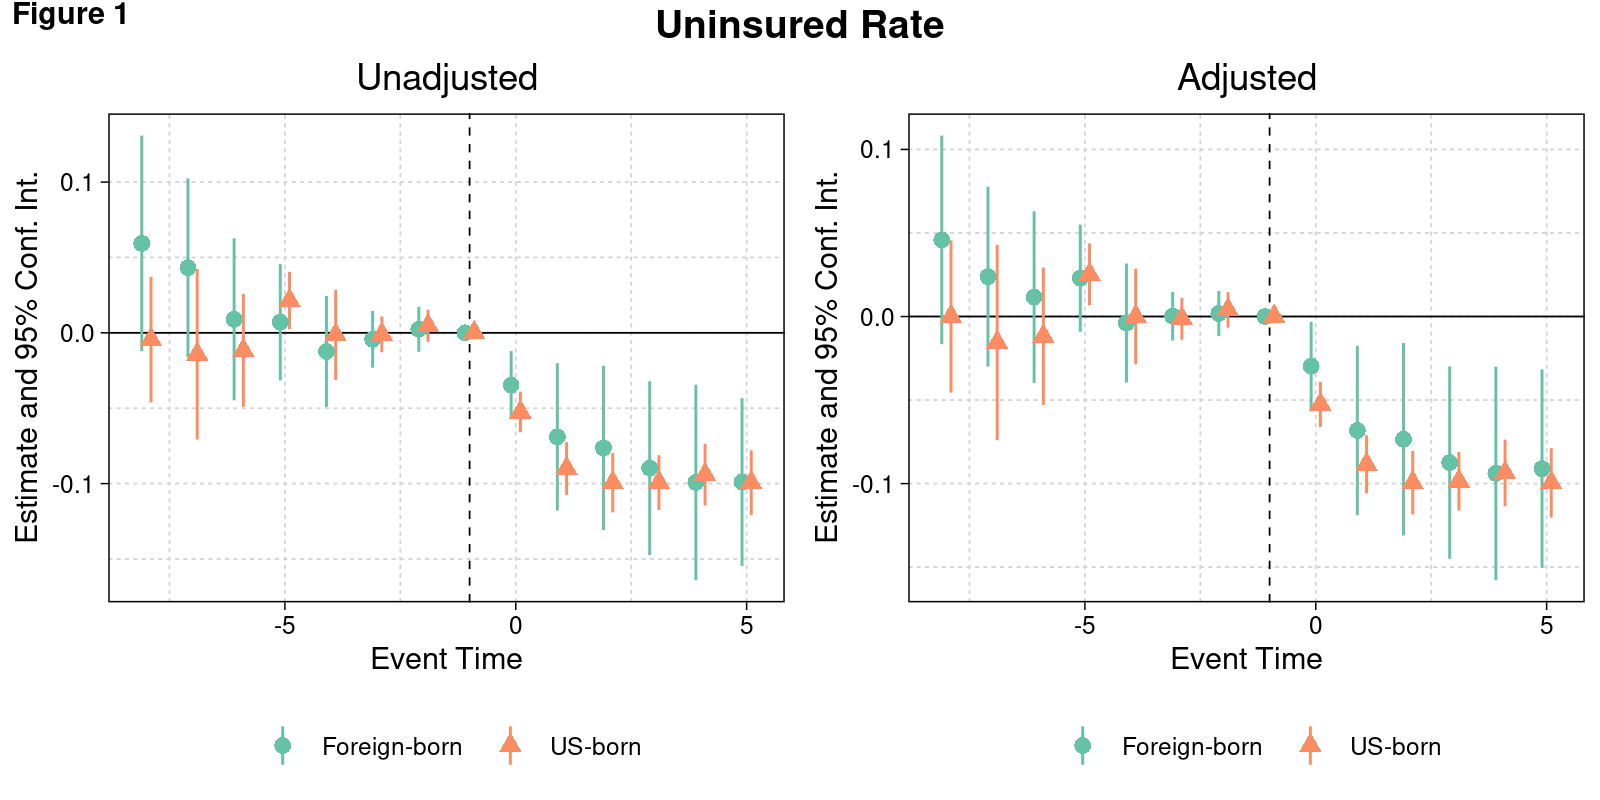
\includegraphics{/home/shadi/Projects/GitHub/medicaid-foreign-born/output/fig1-1} \end{center}

\begin{table}[htbp]
   \caption{The Impact of Medicaid Expansion on Uninsured Rate }
   \centering
   \small
   \renewcommand*{\arraystretch}{0.5}
   \begin{tabular}{lcccc}
      \tabularnewline \midrule \midrule
       & \multicolumn{2}{c}{US-born} & \multicolumn{2}{c}{Foreign-Born} \\ \cmidrule(lr){2-3} \cmidrule(lr){4-5}
      Variables             & (1)            & (2)            & (3)            & (4)\\  
      \midrule 
      expansion year $=$ -8 & -0.005         & 0.0005         & 0.059$^{*}$    & 0.042\\   
                            & (0.021)        & (0.024)        & (0.030)        & (0.024)\\   
      expansion year $=$ -7 & -0.014         & -0.015         & 0.043          & 0.014\\   
                            & (0.025)        & (0.027)        & (0.028)        & (0.022)\\   
      expansion year $=$ -6 & -0.012         & -0.011         & 0.009          & 0.001\\   
                            & (0.019)        & (0.022)        & (0.026)        & (0.025)\\   
      expansion year $=$ -5 & 0.021$^{*}$    & 0.025$^{**}$   & 0.007          & 0.020\\   
                            & (0.011)        & (0.010)        & (0.018)        & (0.016)\\   
      expansion year $=$ -4 & -0.001         & -0.0006        & -0.012         & $9.83\times 10^{-5}$\\    
                            & (0.017)        & (0.017)        & (0.016)        & (0.016)\\   
      expansion year $=$ -3 & -0.001         & -0.001         & -0.004         & -0.002\\   
                            & (0.004)        & (0.005)        & (0.010)        & (0.007)\\   
      expansion year $=$ -2 & 0.005          & 0.004          & 0.002          & -0.010$^{*}$\\   
                            & (0.003)        & (0.004)        & (0.008)        & (0.005)\\   
      expansion year $=$ 0  & -0.052$^{***}$ & -0.053$^{***}$ & -0.035$^{***}$ & -0.029$^{**}$\\   
                            & (0.005)        & (0.005)        & (0.008)        & (0.011)\\   
      expansion year $=$ 1  & -0.090$^{***}$ & -0.088$^{***}$ & -0.069$^{**}$  & -0.065$^{**}$\\   
                            & (0.008)        & (0.008)        & (0.024)        & (0.022)\\   
      expansion year $=$ 2  & -0.100$^{***}$ & -0.100$^{***}$ & -0.076$^{**}$  & -0.066$^{**}$\\   
                            & (0.009)        & (0.009)        & (0.026)        & (0.026)\\   
      expansion year $=$ 3  & -0.099$^{***}$ & -0.099$^{***}$ & -0.090$^{**}$  & -0.083$^{**}$\\   
                            & (0.008)        & (0.008)        & (0.028)        & (0.025)\\   
      expansion year $=$ 4  & -0.094$^{***}$ & -0.094$^{***}$ & -0.099$^{**}$  & -0.092$^{***}$\\   
                            & (0.009)        & (0.009)        & (0.030)        & (0.028)\\   
      expansion year $=$ 5  & -0.100$^{***}$ & -0.101$^{***}$ & -0.099$^{***}$ & -0.072$^{**}$\\   
                            & (0.009)        & (0.009)        & (0.026)        & (0.027)\\   
      State FE              & yes            & yes            & yes            & yes\\  
      Year FE               & yes            & yes            & yes            & yes\\  
      Controls              &                & yes            &                & yes\\  
      Observations          & 1,585,639      & 1,585,639      & 389,955        & 389,955\\  
      R$^2$                 & 0.05930        & 0.11978        & 0.08577        & 0.21554\\  
      Within R$^2$          & 0.00286        & 0.06697        & 0.00172        & 0.14342\\  
      \midrule \midrule
      \multicolumn{5}{l}{\emph{Clustered (State \& Year) standard-errors in parentheses}}\\
      \multicolumn{5}{l}{\emph{Signif. Codes: ***: 0.01, **: 0.05, *: 0.1}}\\
   \end{tabular}
\end{table}

\textbf{Key Observations:}

\begin{itemize}
\item
  Consistent Pre-Trend Patterns:

  \begin{itemize}
  \tightlist
  \item
    For US-born individuals in expansion vs.~non-expansion states;
    coefficients not significantly different from zero.
  \item
    Coefficients for interaction terms between year and pre-treatment
    indicator are small and not statistically significant.
  \end{itemize}
\item
  Witness notable, statistically significant declines in uninsured rates
  for both groups in Post-expansion years
\item
  Notable contrast in lead coefficient shifts for foreign-born compared
  to native individuals, signaling disparities between these groups.
\end{itemize}

\hypertarget{medicaid-coverage}{%
\paragraph{4.3.2. Medicaid Coverage}\label{medicaid-coverage}}

Figure 2 and Table 2, display event-study estimates for unconditional
and conditional parallel trends in Medicaid take-up.

\begin{center}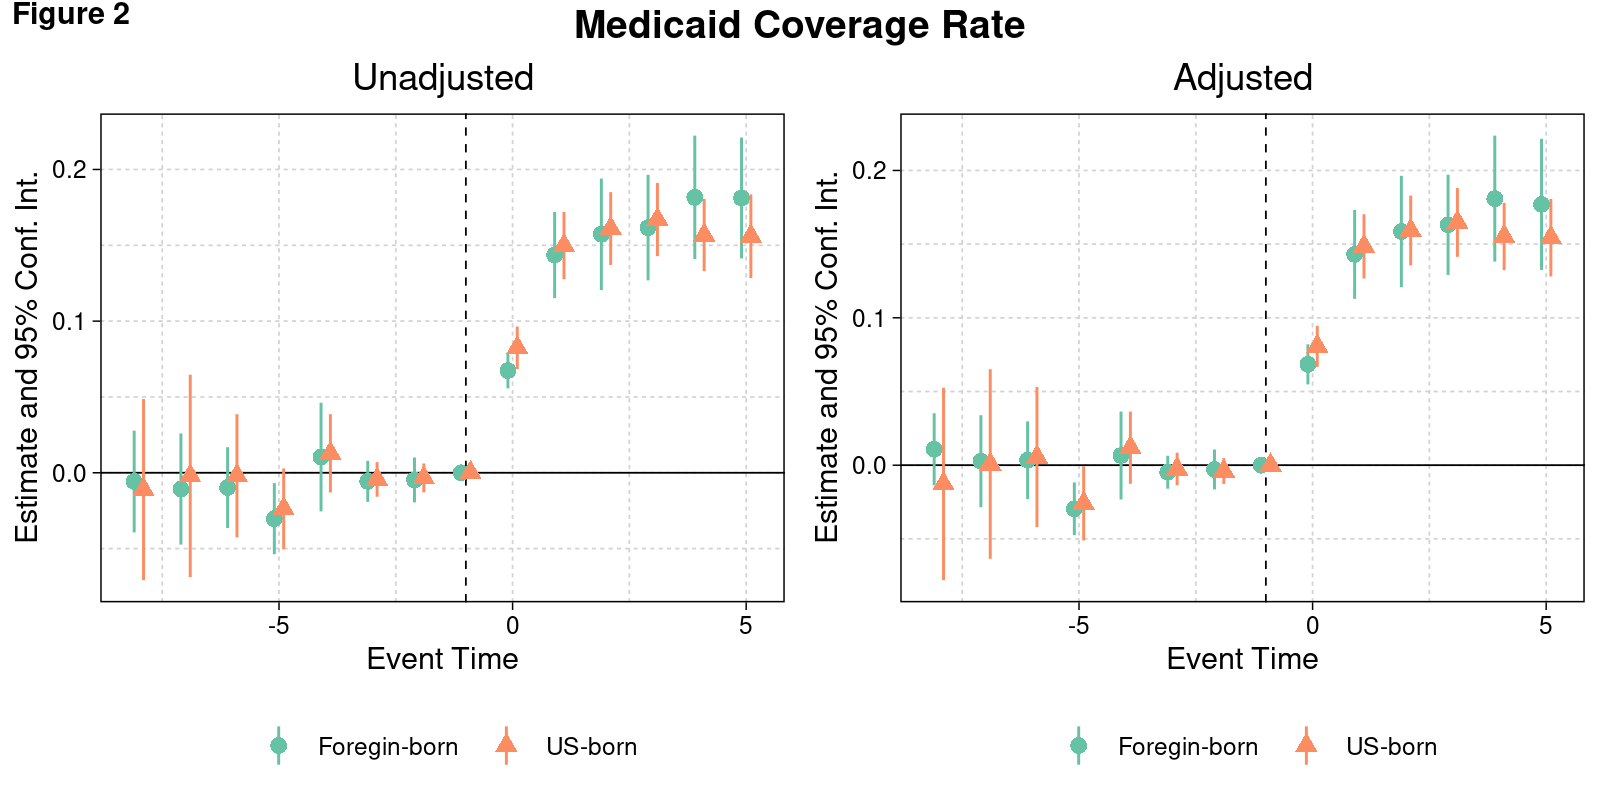
\includegraphics{/home/shadi/Projects/GitHub/medicaid-foreign-born/output/fig2-1} \end{center}

\begin{table}[htbp]
   \caption{The Impact of Medicaid Expansion on Medicaid Coverage }
   \centering
   \small
   \begin{adjustbox}{width = 0.6\textwidth, center}
      \renewcommand*{\arraystretch}{0.5}
      \begin{tabular}{lcccc}
         \tabularnewline \midrule \midrule
          & \multicolumn{2}{c}{US-born} & \multicolumn{2}{c}{Foreign-Born} \\ \cmidrule(lr){2-3} \cmidrule(lr){4-5}
         Variables             & (1)           & (2)           & (3)            & (4)\\  
         \midrule 
         expansion year $=$ -8 & -0.011        & -0.013        & -0.006         & 0.014\\   
                               & (0.029)       & (0.031)       & (0.009)        & (0.010)\\   
         expansion year $=$ -7 & -0.002        & 0.0010        & -0.011         & 0.010\\   
                               & (0.031)       & (0.031)       & (0.013)        & (0.011)\\   
         expansion year $=$ -6 & -0.002        & 0.005         & -0.010         & 0.011\\   
                               & (0.021)       & (0.024)       & (0.011)        & (0.011)\\   
         expansion year $=$ -5 & -0.024        & -0.026$^{*}$  & -0.030$^{***}$ & -0.027$^{***}$\\   
                               & (0.014)       & (0.013)       & (0.008)        & (0.007)\\   
         expansion year $=$ -4 & 0.013         & 0.012         & 0.010          & 0.004\\   
                               & (0.015)       & (0.015)       & (0.017)        & (0.010)\\   
         expansion year $=$ -3 & -0.004        & -0.002        & -0.006         & -0.003\\   
                               & (0.003)       & (0.003)       & (0.006)        & (0.006)\\   
         expansion year $=$ -2 & -0.003        & -0.004        & -0.005         & 0.006\\   
                               & (0.004)       & (0.004)       & (0.007)        & (0.006)\\   
         expansion year $=$ 0  & 0.082$^{***}$ & 0.081$^{***}$ & 0.067$^{***}$  & 0.068$^{***}$\\   
                               & (0.004)       & (0.005)       & (0.002)        & (0.005)\\   
         expansion year $=$ 1  & 0.150$^{***}$ & 0.148$^{***}$ & 0.144$^{***}$  & 0.141$^{***}$\\   
                               & (0.011)       & (0.011)       & (0.013)        & (0.012)\\   
         expansion year $=$ 2  & 0.161$^{***}$ & 0.159$^{***}$ & 0.157$^{***}$  & 0.153$^{***}$\\   
                               & (0.011)       & (0.012)       & (0.017)        & (0.014)\\   
         expansion year $=$ 3  & 0.167$^{***}$ & 0.165$^{***}$ & 0.162$^{***}$  & 0.160$^{***}$\\   
                               & (0.011)       & (0.012)       & (0.017)        & (0.014)\\   
         expansion year $=$ 4  & 0.157$^{***}$ & 0.155$^{***}$ & 0.182$^{***}$  & 0.180$^{***}$\\   
                               & (0.010)       & (0.010)       & (0.018)        & (0.019)\\   
         expansion year $=$ 5  & 0.156$^{***}$ & 0.154$^{***}$ & 0.181$^{***}$  & 0.164$^{***}$\\   
                               & (0.011)       & (0.011)       & (0.017)        & (0.017)\\   
         State FE              & yes           & yes           & yes            & yes\\  
         Year FE               & yes           & yes           & yes            & yes\\  
         Controls              &               & yes           &                & yes\\  
         Observations          & 1,585,639     & 1,585,639     & 389,955        & 389,955\\  
         R$^2$                 & 0.06514       & 0.18770       & 0.10655        & 0.18067\\  
         Within R$^2$          & 0.00628       & 0.13656       & 0.00837        & 0.09064\\  
         \midrule \midrule
         \multicolumn{5}{l}{\emph{Clustered (State \& Year) standard-errors in parentheses}}\\
         \multicolumn{5}{l}{\emph{Signif. Codes: ***: 0.01, **: 0.05, *: 0.1}}\\
      \end{tabular}
   \end{adjustbox}
\end{table}

\textbf{Key Observations:}

\begin{itemize}
\item
  No Pre-Trend Differences: Before Medicaid expansion, no significant
  differences observed in Medicaid take-up between expansion and
  non-expansion states for low-income US-born and foreign-born
  individuals (26-64).
\item
  Interaction term coefficients small and statistically insignificant,
  indicating no pre-trend disparity in uninsured rates between expansion
  and non-expansion states.
\item
  Coefficients for post-treatment years (0 to 5 after expansion)
  positive and statistically significant in all models, showing
  increased Medicaid coverage in expansion states.
\item
  Observed divergence in Take-Up Trends: Over time, foreign-born
  individuals' Medicaid take-up increased, differing from US-born
  individuals; potential factors include policy changes, targeted
  outreach, or specific programs.
\item
  Demonstrates Medicaid expansion's effectiveness in enhancing
  healthcare access, particularly among foreign-born individuals.
\end{itemize}

\hypertarget{difference-in-differences}{%
\subsubsection{4.4.
Difference-in-Differences}\label{difference-in-differences}}

\textbf{Uninsured Rate}

\begin{table}[htbp]
   \centering
   \begin{threeparttable}[b]
      \caption{The Effect of Medicaid Expansion on Uninsured Rate (Difference-in-Differences Estimation)}
      \begin{tabular}{lccccc}
         \tabularnewline \midrule \midrule
                                                         & (1)            & (2)            & (3)            & (4)            & (5)\\  
         \midrule 
         Medicaid Expansion                              & -0.075$^{***}$ & -0.081$^{***}$ & -0.092$^{***}$ & -0.084$^{***}$ & -0.095$^{***}$\\   
                                                         & (0.002)        & (0.002)        & (0.002)        & (0.002)        & (0.002)\\   
         Foreign-Born                                    & 0.244$^{***}$  & 0.018$^{*}$    & 1.10$^{***}$   & 0.051$^{***}$  & 0.995$^{***}$\\   
                                                         & (0.001)        & (0.010)        & (0.062)        & (0.014)        & (0.074)\\   
         Medicaid Expansion $\times$ Foreign-Born        & -0.031$^{***}$ & 0.0010         & 0.004$^{*}$    & 0.017$^{***}$  & 0.021$^{***}$\\   
                                                         & (0.002)        & (0.002)        & (0.002)        & (0.003)        & (0.003)\\   
         State Political Ideology                        &                & -0.028$^{***}$ & -0.003         & -0.018$^{**}$  & 0.007\\   
                                                         &                & (0.007)        & (0.008)        & (0.007)        & (0.008)\\   
         Foreign-Born $\times$ State Political Ideology  &                &                &                & -0.089$^{***}$ & -0.092$^{***}$\\   
                                                         &                &                &                & (0.006)        & (0.006)\\   
         \midrule 
         Controls x Foreign-born                         & No             & No             & No             & Yes            & Yes\\  
         Controls                                        &                & yes            & yes            & yes            & yes\\  
         State and Year FE                               & yes            & yes            & yes            & yes            & yes\\  
         Region-Year FE                                  &                &                & yes            &                & yes\\  
         \midrule 
         Standard-Errors & \multicolumn{5}{c}{Heteroskedasticity-robust} \\ 
         Observations                                    & 1,975,594      & 1,975,594      & 1,975,594      & 1,975,594      & 1,975,594\\  
         R$^2$                                           & 0.10174        & 0.17712        & 0.17423        & 0.17820        & 0.17689\\  
         Within R$^2$                                    & 0.04288        & 0.12320        & 0.11887        & 0.12435        & 0.12171\\  
         \midrule \midrule
         \multicolumn{6}{l}{\emph{Heteroskedasticity-robust standard-errors in parentheses}}\\
         \multicolumn{6}{l}{\emph{Signif. Codes: ***: 0.01, **: 0.05, *: 0.1}}\\
      \end{tabular}
   \end{threeparttable}
\end{table}

\textbf{Key Observations:}

\begin{itemize}
\tightlist
\item
  Model 4 stands out as the best-fitting model according to R2 results.
\item
  The incorporation of interaction terms for control variables differing
  between foreign-born and native individuals appears to have enhanced
  model fit.
\item
  Medicaid Expansion notably reduced the probability of being uninsured.
\item
  Being foreign-born correlates with an increased chance of being
  uninsured, though the extent varies across different models.
\item
  The significance and direction of coefficients for Medicaid Expansion
  x Foreign-Born interactions differ across models.

  \begin{itemize}
  \tightlist
  \item
    In Model 1, the negative and significant coefficient implies a
    smaller uninsured probability for foreign-born individuals compared
    to US-born.
  \item
    In Model 2, the coefficient lacks significance, suggesting no
    distinct difference in uninsured probabilities.
  \item
    In Models 3 to 5, the positive coefficient signifies a reduced
    impact of Medicaid expansion on decreasing the uninsured rate for
    foreign-born individuals relative to US-born individuals.
  \end{itemize}
\item
  Model 3 features a coefficient exceeding 1, rendering it unsuitable
  for meaningful interpretation due to the linear probability
  framework's limitations.
\item
  While the heatmap hinted at differences in outcomes by region and
  year, adding a Region-year fixed effect in the later analysis didn't
  show any clear improvements in model fit.
\end{itemize}

\textbf{Medicaid Coverage}

\begin{table}[htbp]
   \centering
   \begin{threeparttable}[b]
      \caption{The Effect of Medicaid Expansion on Uninsured Rate (Difference-in-Differences Estimation)}
      \begin{tabular}{lccccc}
         \tabularnewline \midrule \midrule
                                                         & (1)            & (2)            & (3)            & (4)            & (5)\\  
         \midrule 
         Medicaid Expansion                              & 0.136$^{***}$  & 0.140$^{***}$  & 0.148$^{***}$  & 0.144$^{***}$  & 0.151$^{***}$\\   
                                                         & (0.002)        & (0.002)        & (0.002)        & (0.002)        & (0.002)\\   
         Foreign-Born                                    & -0.158$^{***}$ & -0.098$^{***}$ & 0.011          & 0.012          & 0.192$^{***}$\\   
                                                         & (0.001)        & (0.010)        & (0.059)        & (0.014)        & (0.071)\\   
         Medicaid Expansion $\times$ Foreign-Born        & 0.007$^{***}$  & -0.012$^{***}$ & -0.015$^{***}$ & -0.032$^{***}$ & -0.036$^{***}$\\   
                                                         & (0.002)        & (0.002)        & (0.002)        & (0.002)        & (0.003)\\   
         State Political Ideology                        &                & -0.010         & -0.049$^{***}$ & -0.023$^{***}$ & -0.062$^{***}$\\   
                                                         &                & (0.008)        & (0.008)        & (0.008)        & (0.008)\\   
         Foreign-Born $\times$ State Political Ideology  &                &                &                & 0.105$^{***}$  & 0.108$^{***}$\\   
                                                         &                &                &                & (0.006)        & (0.006)\\   
         \midrule 
         Controls x Foreign-born                         & No             & No             & No             & Yes            & Yes\\  
         Controls                                        &                & yes            & yes            & yes            & yes\\  
         State and Year FE                               & yes            & yes            & yes            & yes            & yes\\  
         Region-Year FE                                  &                &                & yes            &                & yes\\  
         \midrule 
         Standard-Errors & \multicolumn{5}{c}{Heteroskedasticity-robust} \\ 
         Observations                                    & 1,975,594      & 1,975,594      & 1,975,594      & 1,975,594      & 1,975,594\\  
         R$^2$                                           & 0.08522        & 0.19213        & 0.19214        & 0.19494        & 0.19386\\  
         Within R$^2$                                    & 0.02242        & 0.13666        & 0.13407        & 0.13967        & 0.13591\\  
         \midrule \midrule
         \multicolumn{6}{l}{\emph{Heteroskedasticity-robust standard-errors in parentheses}}\\
         \multicolumn{6}{l}{\emph{Signif. Codes: ***: 0.01, **: 0.05, *: 0.1}}\\
      \end{tabular}
   \end{threeparttable}
\end{table}

\textbf{Key Observations:}

\begin{itemize}
\item
  The incorporation of interaction terms for control variables differing
  between foreign-born and native individuals appears to have enhanced
  model fit.
\item
  Model 4 stands out as the best-fitting model according to R2 results.
\item
  Medicaid Expansion notably increased the probability of having
  medicaid coverage for low income aged 26-64.
\item
  In Model 1 and 2, the coefficient for ``Foreign-Born'' is negative,
  indicating that being foreign-born is associated with a decrease in
  the probability of having Medicaid coverage However, in subsequent
  models (Model 4 and Model 5), the coefficient for ``Foreign-Born''
  becomes positive (0.011 to 0.192). This implies that the effect of
  being foreign-born on Medicaid coverage is not consistently negative
  and could be postive or have no effect based on other factors in the
  model.
\item
  The interaction effect term ``Medicaid Expansion x Foreign-Born''
  suggests that the impact of Medicaid Expansion on Medicaid coverage
  changes based on foreign-born status. Model indicating a slight
  increase in the impact of Medicaid Expansion for foreign-born
  individuals However, in subsequent models (Model 3 to Model 5), the
  coefficient becomes negative (-0.015 to -0.036). This suggests that
  the effect of Medicaid Expansion diminishes for foreign-born
  individuals as other factors are considered.
\item
  Being foreign-born correlates with the chance of having a med, though
  the extent varies across different models.
\item
  The significance and direction of coefficients for Medicaid Expansion
  x Foreign-Born interactions differ across models.

  \begin{itemize}
  \tightlist
  \item
    In Model 1, the negative and significant coefficient implies a
    smaller uninsured probability for foreign-born individuals compared
    to US-born.
  \item
    In Model 2, the coefficient lacks significance, suggesting no
    distinct difference in uninsured probabilities.
  \item
    In Models 3 to 5, the positive coefficient signifies a reduced
    impact of Medicaid expansion on decreasing the uninsured rate for
    foreign-born individuals relative to US-born individuals.
  \end{itemize}
\item
  Model 3 features a coefficient exceeding 1, rendering it unsuitable
  for meaningful interpretation due to the linear probability
  framework's limitations.
\item
  While the heatmap hinted at differences in outcomes by region and
  year, adding a Region-year fixed effect in the later analysis didn't
  show any clear improvements in model fit.
\end{itemize}

\hypertarget{addressing-threat-of-treatment-heterogenity}{%
\subsubsection{4.5. Addressing Threat of Treatment
Heterogenity}\label{addressing-threat-of-treatment-heterogenity}}

\hypertarget{sun-abraham-interaction-weighted-iw-event-study}{%
\paragraph{4.5.1. Sun \& Abraham Interaction-weighted (IW) event
study}\label{sun-abraham-interaction-weighted-iw-event-study}}

Since 2018, there's been a growing focus on validating staggered
Difference-in-Differences (DID) models and event study designs.To
address these concerns and account for heterogeneous treatment effects,
we use the interaction-weighted (IW) event study estimator by Sun and
Abraham (2021).

\begin{center}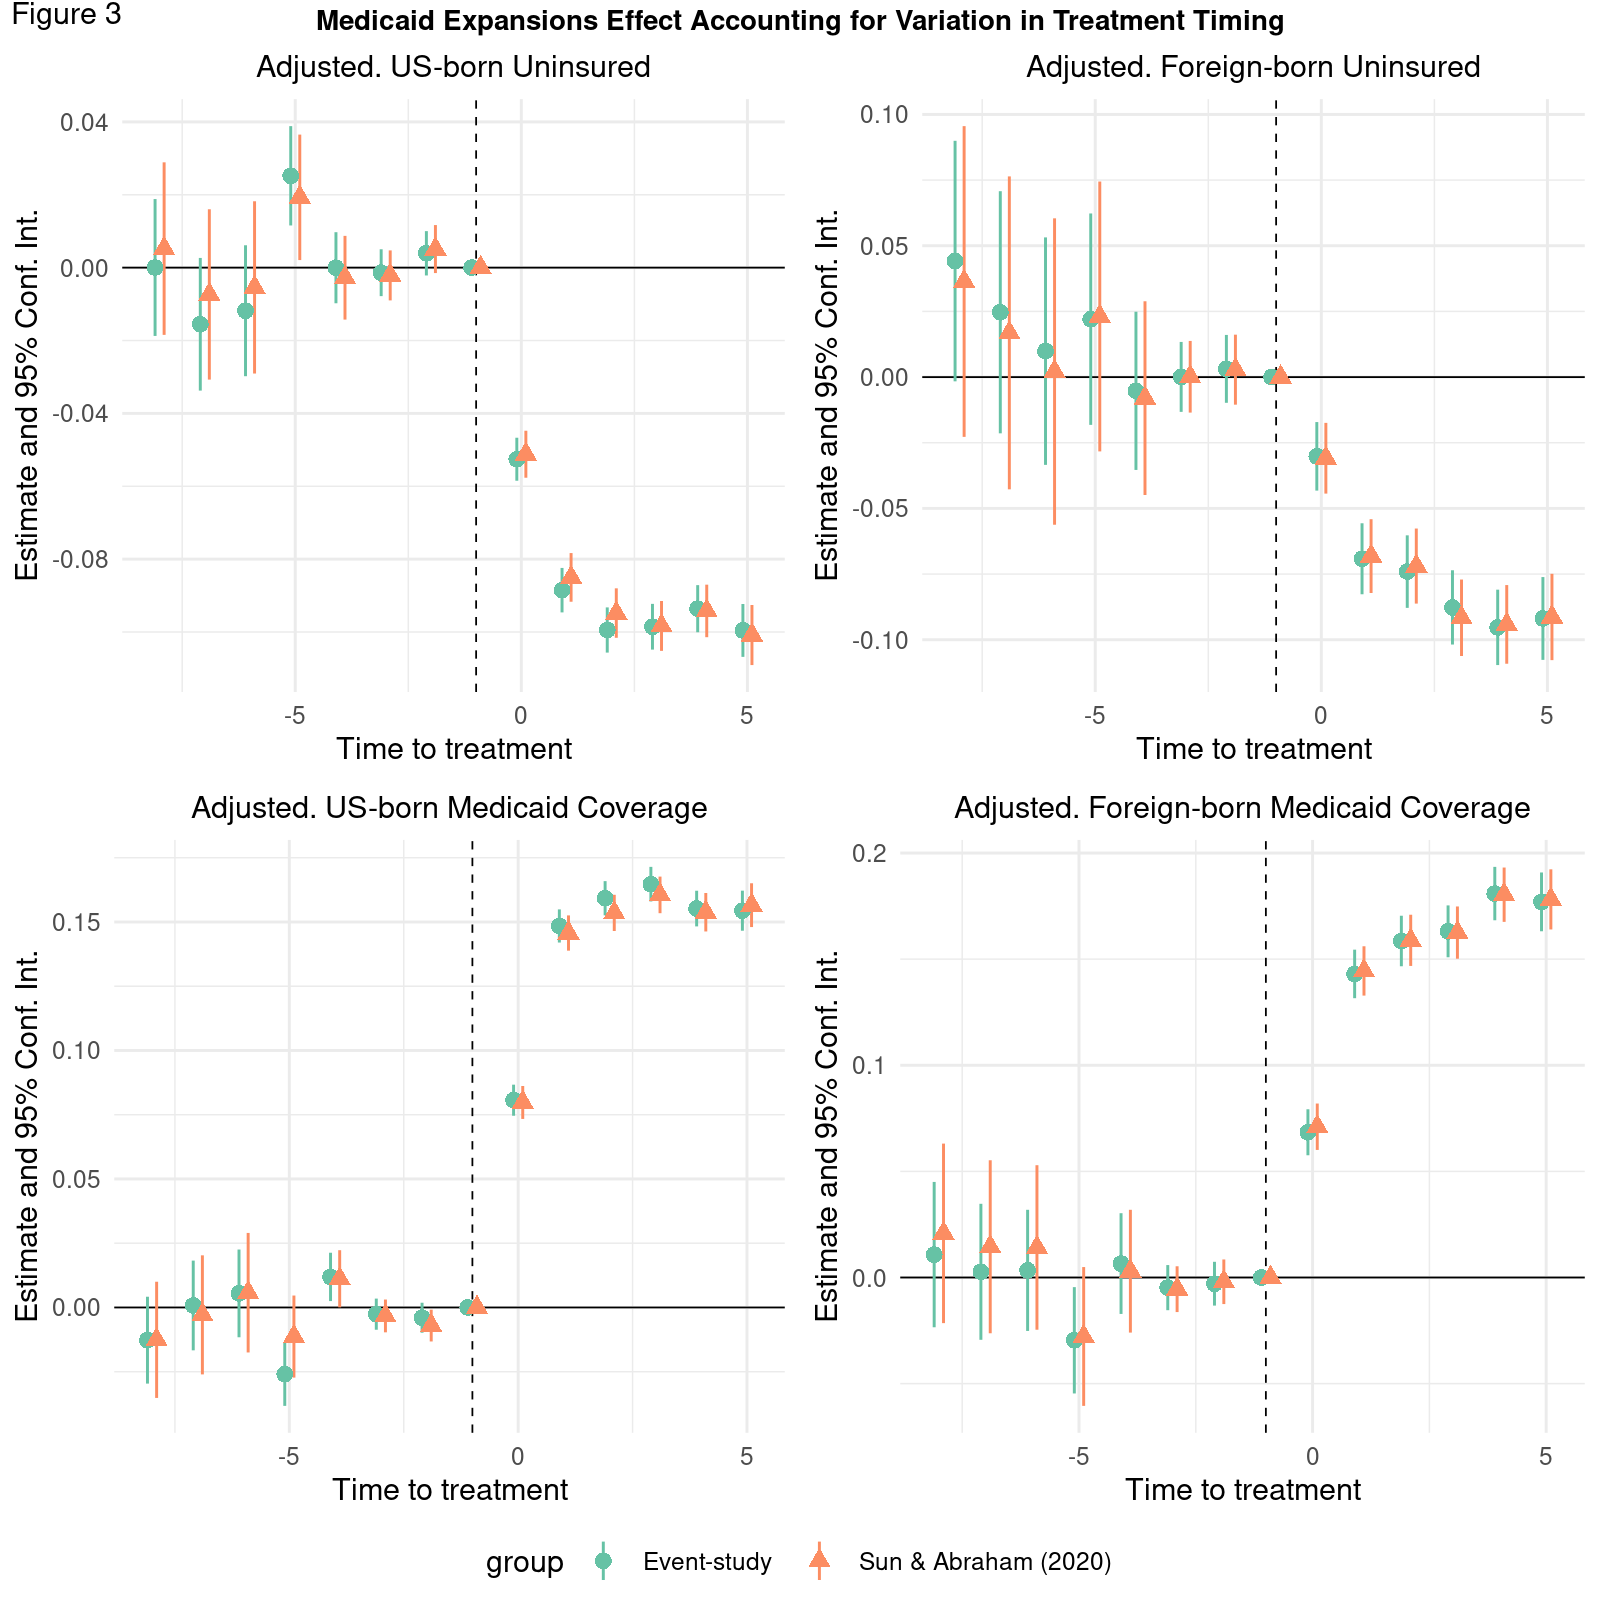
\includegraphics{/home/shadi/Projects/GitHub/medicaid-foreign-born/output/sun&abr-1} \end{center}

\begin{itemize}
\tightlist
\item
  No evidence of differing pre-trends is found, we can conclude our
  results are robust and not disproportionately influenced by variations
  in treatment effects across diverse cohorts.
\end{itemize}

\hypertarget{bacon-decomposition}{%
\paragraph{4.5.2. Bacon decomposition}\label{bacon-decomposition}}

\begin{itemize}
\tightlist
\item
  Compares timing groups to untreated units and evaluates relative
  treatment effects at different timings.
\end{itemize}

\begin{table}

\caption{\label{tab:tab9}Bacon Decomposition}
\centering
\begin{tabular}[t]{lll}
\toprule
Comparison & Coefficient & Weight\\
\midrule
\addlinespace[1em]
\multicolumn{3}{l}{\textbf{Uninsured}}\\
\hspace{1em}Earlier vs Later Treated & -0.09309 & 0.11871\\
\hspace{1em}Later vs Earlier Treated & -0.05521 & 0.08771\\
\hspace{1em}Treated vs Untreated & -0.08462 & 0.79358\\
\addlinespace[0.3em]
\multicolumn{3}{l}{\textbf{Medicaid}}\\
\hspace{1em}Earlier vs Later Treated & 0.14610 & 0.11871\\
\hspace{1em}Later vs Earlier Treated & 0.08782 & 0.08771\\
\hspace{1em}Treated vs Untreated & 0.14452 & 0.79358\\
\bottomrule
\end{tabular}
\end{table}

\begin{center}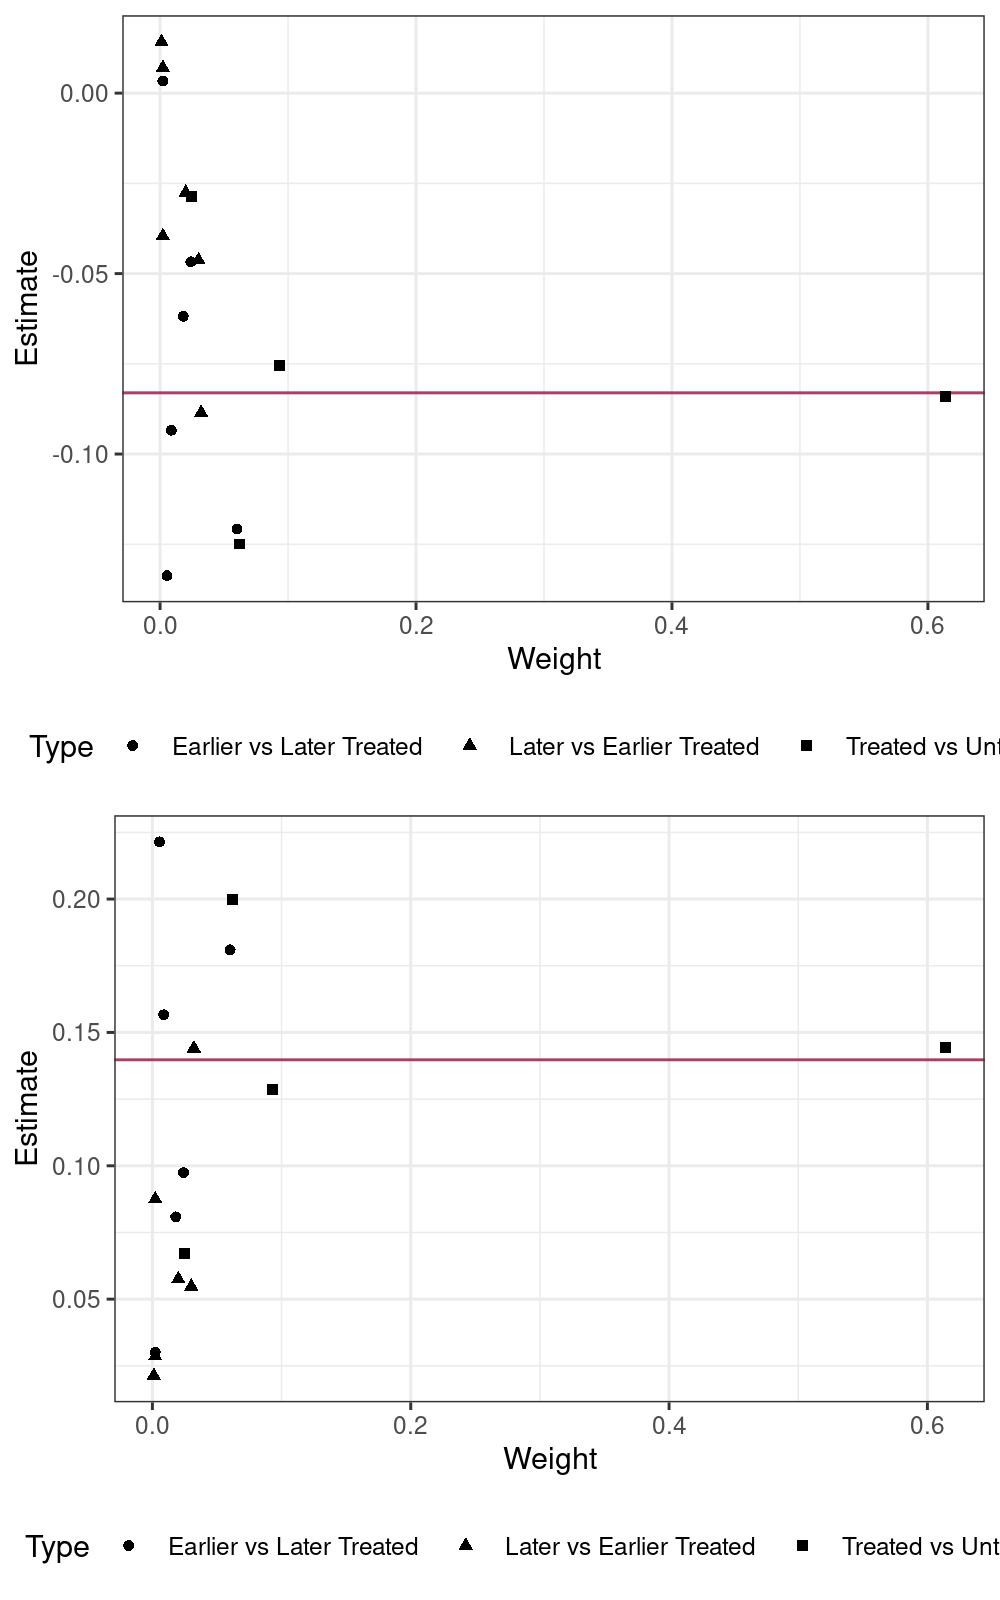
\includegraphics{/home/shadi/Projects/GitHub/medicaid-foreign-born/output/plotbac-1} \end{center}

\begin{itemize}
\item
  When we exclude variation due to state-level treatment timing
  differences:

  \begin{itemize}
  \tightlist
  \item
    Difference-in-Differences (DD) estimate remains highly consistent
    with main DD estimate.
  \item
    Treatment effect magnitude from 2014 wave aligns with subsequent
    wave effects.
  \end{itemize}
\item
  Result Confirms the reliability of the estimated treatment effect.
\item
  Figure 4 illustrates 2 × 2 DD estimates and associated weights.
\end{itemize}

\end{document}
